% =====================================================================
%  8. Diagnostics et explicabilité
% =====================================================================
\clearpage
\section{Diagnostics des performances et explicabilité}
\label{sec:diag}

Le premier benchmark (\cref{tab:bench13}) a produit des $R^2$ faibles en
validation groupée. Plutôt que d'essayer des modèles au hasard, le notebook
\notebook{04\_diagnostics.ipynb} a cherché à \emph{comprendre} ces scores. Le
protocole des diagnostics a été fixé avant leur calcul ; il réutilise les mêmes
labels, la même cohorte et les mêmes plis. Ces analyses sont \textbf{rétrospectives} :
elles ne constituent pas une validation indépendante des choix qu'elles ont motivés.

\subsection{Les modèles apprennent, mais transfèrent mal}

Le \cref{tab:ecart_train} compare les scores sur le train et en validation
groupée pour le benchmark 13/itérative.

\begin{table}[htbp]
\centering
\small
\caption{Écart entre entraînement et validation groupée, forêt aléatoire du benchmark 13/itérative.}
\label{tab:ecart_train}
\begin{tabular}{@{}lrrrr@{}}
\toprule
Cible & MAE train & MAE validation & $R^2$ train & $R^2$ validation \\
\midrule
\YS{} (MPa)             & 30,08 & 65,88 & 0,795 & 0,079 \\
\UTS{} (MPa)            & 23,79 & 57,65 & 0,842 & 0,194 \\
Allongement (pts de \%) & 1,33  & 3,56  & 0,859 & 0,125 \\
\charpy{} (J)           & 8,40  & 34,71 & 0,941 & 0,017 \\
\bottomrule
\end{tabular}
\end{table}

La forêt reproduit bien le train ($R^2$ de 0,80 à 0,94) mais généralise mal aux
séries absentes. Les modèles linéaires ont aussi un faible $R^2$ d'entraînement
(0,18 à 0,27 pour Ridge) : ajouter de la capacité non linéaire ne suffit pas.
De plus, les prédictions sont \textbf{comprimées} : l'écart-type des prédictions
vaut environ 0,53 fois celui des observations pour \YS{} et Charpy, 0,68 pour
\UTS{} et 0,64 pour l'allongement ; les soudures très résistantes ou très
tenaces sont sous-estimées.

\subsection{Une grande part de l'erreur vient des séries}

L'erreur quadratique totale peut se décomposer exactement en une part due au
\textbf{biais moyen de chaque série} et une part due aux variations à
l'intérieur des séries :
\begin{equation}
  \mathrm{SSE} = \sum_{g}\sum_{i \in g} e_i^2
  = \underbrace{\sum_{g} n_g\, b_g^2}_{\text{décalage des séries}}
  + \underbrace{\sum_{g}\sum_{i \in g}\bigl(e_i - b_g\bigr)^2}_{\text{dispersion interne}},
\end{equation}
où $e_i = \hat{y}_i - y_i$ est l'erreur de la ligne $i$, $n_g$ l'effectif de la
série $g$ et $b_g = \frac{1}{n_g}\sum_{i\in g} e_i$ son biais moyen.

\begin{table}[htbp]
\centering
\small
\caption{Décomposition de l'erreur de la forêt du benchmark 13/itérative (prédictions OOF réunies).}
\label{tab:decomposition}
\begin{tabularx}{\textwidth}{@{}l C C C C C@{}}
\toprule
Cible & Variance entre séries (\% de SST) & Part de SSE due au biais des séries & $R^2$ OOF & RMSE OOF & RMSE requise pour $R^2 = 0{,}5$ \\
\midrule
\YS{} (MPa)       & 48,0\,\% & 56,4\,\% & 0,091 & 87,7 & 65,0 \\
\UTS{} (MPa)      & 54,9\,\% & 50,6\,\% & 0,280 & 75,9 & 63,3 \\
Allongement (pts) & 54,4\,\% & 50,0\,\% & 0,156 & 4,48 & 3,45 \\
\charpy{} (J)     & 29,1\,\% & 36,5\,\% & 0,116 & 47,5 & 35,7 \\
\bottomrule
\end{tabularx}
\end{table}

Le \cref{tab:decomposition} montre que \textbf{la moitié environ de l'erreur
quadratique} provient de décalages de niveau entre séries : le modèle se trompe
de façon systématique sur une série entière. La \cref{fig:biais} donne les séries
qui concentrent le plus d'erreur. Les biais sont majoritairement négatifs pour la
résistance : les séries très résistantes (par exemple \texttt{SurianEtAl-C-1991},
\texttt{Birmingham}, \texttt{Sw\&Rog-1973}) sont sous-estimées de 170 à 240\,MPa.

\begin{figure}[htbp]
\centering
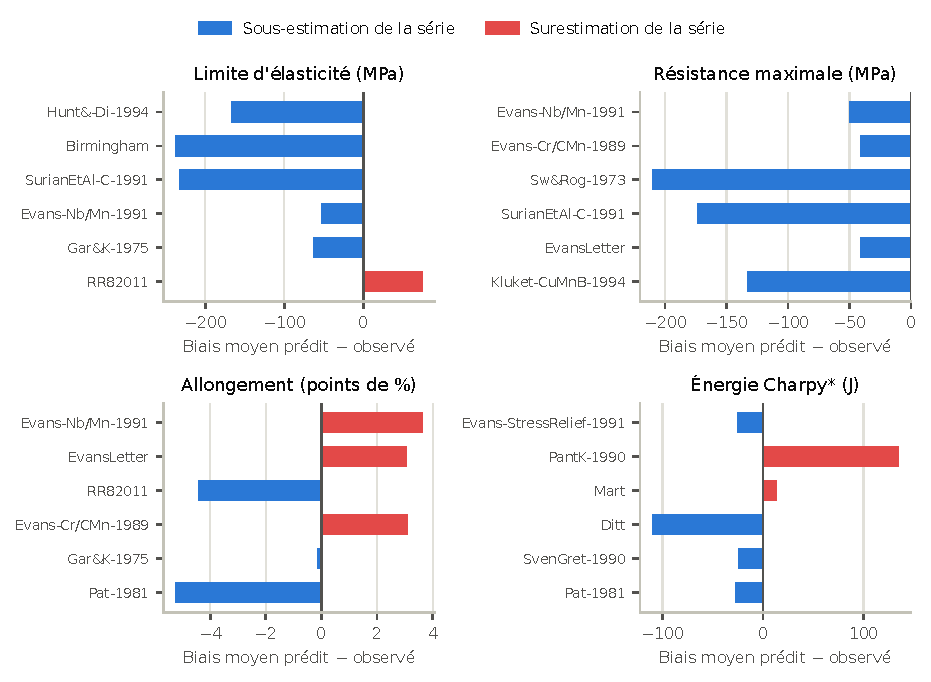
\includegraphics[width=\textwidth]{diag_biais_series}
\caption{Biais moyen (prédit $-$ observé) des six séries qui contribuent le plus à
l'erreur quadratique, forêt du benchmark 13/itérative, validation groupée.}
\label{fig:biais}
\end{figure}

L'examen de cas concrets éclaire ces décalages. La ligne 722
(\texttt{Evans-AlEl9Cr1Mo-1994}) contient 3,01\,\% de Ni et 9,17\,\% de Cr ; son
\UTS{} observée vaut 1\,151\,MPa contre 729\,MPa prédits. La ligne 1\,209
(\texttt{PantK-1990}) contient 8,7\,\% de Cr ; son énergie Charpy observée est de
8\,J contre 159\,J prédits. Or Ni, Cr et Mo \emph{ne faisaient pas partie} des
13 entrées. Ces exemples suggèrent une information omise, que l'extension à
16 entrées teste directement (\cref{subsec:sensibilites}).

\subsection{Domaine des entrées et rôle de l'imputation}

Le \cref{tab:domaine} compare la MAE selon trois indicateurs : présence d'une
entrée imputée, entrée hors des plages observées dans le train, procédé absent
du train.

\begin{table}[htbp]
\centering
\small
\caption{MAE de la forêt (benchmark 13/itérative) selon l'appartenance au domaine du train.}
\label{tab:domaine}
\begin{tabular}{@{}l rr rr rr@{}}
\toprule
 & \multicolumn{2}{c}{Entrée imputée} & \multicolumn{2}{c}{Hors plages du train} & \multicolumn{2}{c}{Procédé inconnu} \\
\cmidrule(lr){2-3}\cmidrule(lr){4-5}\cmidrule(lr){6-7}
Cible & non & oui & non & oui & non & oui \\
\midrule
\YS{} (MPa)       & 72,5 & 57,4 & 65,0 & 73,2 & 64,4 & 102,4 \\
\UTS{} (MPa)      & 58,5 & 53,5 & 54,9 & 64,0 & 54,6 & 95,3 \\
Allongement (pts) & 3,64 & 3,44 & 3,67 & 2,99 & 3,50 & 4,29 \\
\charpy{} (J)     & 33,5 & 37,1 & 28,2 & 52,8 & 32,9 & 45,2 \\
\bottomrule
\end{tabular}
\end{table}

Deux constats en ressortent. D'abord, les lignes avec une entrée imputée
\textbf{ne sont pas systématiquement moins bien prédites} ; pour \YS{} elles le
sont même mieux. L'hypothèse \og l'imputation explique tout \fg{} est donc
contredite. Ensuite, sortir du domaine du train dégrade nettement Charpy
(MAE de 52,8\,J contre 28,2\,J, corrélation de rang erreur/distance 0,41), et un
procédé inconnu du train dégrade fortement \YS{} et \UTS{} (MAE
d'environ 100\,MPa). Ces comparaisons sont descriptives et confondues par les
séries.

\subsection{Sensibilités : entrées et méthode d'imputation}
\label{subsec:sensibilites}

Pour isoler les deux facteurs (nombre d'entrées et imputation), les six
combinaisons \{11, 13, 16 entrées\} $\times$ \{médiane, itérative\} ont été
évaluées avec les quatre familles, les grilles du notebook 03 et les mêmes plis
groupés : 480 évaluations prévues. \textbf{436 ont abouti} ; l'imputation
itérative à 16 entrées \textbf{n'a pas convergé} dans 11 contextes cible/pli
(\YS{} pli 4 ; \UTS{} plis 3--4 ; allongement plis 2--4 ; Charpy tous les plis),
rendant 44 évaluations indisponibles. Conformément au protocole, aucun repli
silencieux n'a été appliqué.

\begin{figure}[htbp]
\centering
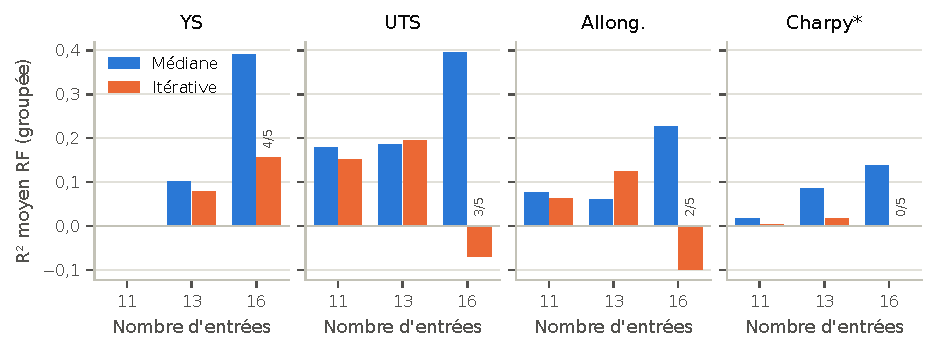
\includegraphics[width=\textwidth]{diag_sensibilites_rf}
\caption{$R^2$ moyen de la forêt aléatoire en validation groupée selon le nombre
d'entrées et l'imputation. Les mentions \og $k$/5 \fg{} signalent les scénarios
où seuls $k$ plis sur 5 ont abouti (non comparables aux scénarios complets).}
\label{fig:sensibilites}
\end{figure}

\begin{table}[htbp]
\centering
\small
\caption{Forêt aléatoire en validation groupée : MAE et $R^2$ moyens selon le
schéma et l'imputation (plis aboutis sur 5 entre parenthèses lorsque incomplets).}
\label{tab:sensibilites}
\setlength{\tabcolsep}{4.5pt}
\begin{tabular}{@{}l l rr rr rr rr@{}}
\toprule
 & & \multicolumn{2}{c}{\YS{} (MPa)} & \multicolumn{2}{c}{\UTS{} (MPa)} & \multicolumn{2}{c}{Allong. (pts)} & \multicolumn{2}{c}{\charpy{} (J)} \\
\cmidrule(lr){3-4}\cmidrule(lr){5-6}\cmidrule(lr){7-8}\cmidrule(lr){9-10}
Entrées & Imputation & MAE & $R^2$ & MAE & $R^2$ & MAE & $R^2$ & MAE & $R^2$ \\
\midrule
11 & médiane   & 68,98 & 0,000 & 57,31 & 0,179 & 3,69 & 0,076 & 35,14 & 0,018 \\
11 & itérative & 69,14 & $-0{,}001$ & 58,38 & 0,151 & 3,68 & 0,063 & 34,71 & 0,002 \\
13 & médiane   & 64,98 & 0,102 & 57,84 & 0,185 & 3,74 & 0,060 & 33,70 & 0,084 \\
13 & itérative & 65,88 & 0,079 & 57,65 & 0,194 & 3,56 & 0,125 & 34,71 & 0,017 \\
16 & médiane   & \meilleur{54,14} & \meilleur{0,390} & \meilleur{48,91} & \meilleur{0,394} & \meilleur{3,34} & \meilleur{0,226} & \meilleur{33,03} & \meilleur{0,138} \\
16 & itérative & 60,80 (4) & 0,156 & 57,32 (3) & $-0{,}069$ & 3,97 (2) & $-0{,}099$ & -- (0) & -- \\
\bottomrule
\end{tabular}
\end{table}

Le passage de 13 à 16 entrées à imputation médiane identique produit un
\textbf{gain apparié de MAE OOF} de la forêt (bootstrap par groupes, 2\,000 tirages) :
\begin{itemize}
  \item \YS{} : \textbf{11,06\,MPa}, intervalle [3,09 ; 20,19] ;
  \item \UTS{} : \textbf{8,80\,MPa}, intervalle [2,38 ; 15,40] ;
  \item allongement : 0,39 point, intervalle [$-0{,}05$ ; 0,87] ;
  \item Charpy : 0,65\,J, intervalle [$-0{,}21$ ; 1,64].
\end{itemize}
Les intervalles de \YS{} et \UTS{} excluent zéro : Ni, Cr et Mo apportent une
information prédictive réelle sur la résistance. Pour l'allongement et Charpy,
le gain n'est pas établi.

Un contrôle complémentaire a masqué 20\,\% des valeurs \emph{observées} de Ni,
Cr et Mo en validation, puis comparé leur reconstruction. L'itérative ne domine
pas : pour Charpy, l'erreur absolue moyenne sur Cr vaut 4,79\,\% massique avec
l'itérative contre 1,50\,\% avec la médiane, sur les mêmes cellules. Une
imputation plus sophistiquée ne garantit donc pas une meilleure reconstruction
hors série.

\begin{decision}
La configuration de travail devient \textbf{16 entrées + médiane} : gain établi
pour \YS{} et \UTS, convergence garantie, aucune perte de lignes. Elle reste un
\emph{candidat} à valider sur des séries indépendantes, car elle a été choisie
après observation des scores.
\end{decision}

\paragraph{Sélection conjointe interne.} Pour mesurer ce que coûterait un choix
automatique, une procédure a aussi choisi \emph{dans la boucle interne} le schéma,
l'imputation, la famille et les hyperparamètres. Ses $R^2$ externes sont 0,337
(\YS), 0,334 (\UTS), 0,164 (allongement) et $-0{,}100$ (Charpy), inférieurs à ceux
de la forêt 16/médiane fixée : la sélection fluctue d'un pli à l'autre, signe
de la fragilité du transfert. Enfin, régler les hyperparamètres par MSE plutôt
que par MAE ne change presque rien (par exemple $R^2$ de la forêt pour \UTS{} :
0,206 contre 0,194).

\subsection{Effet du mode de découpage}
\label{subsec:decoupages}

Si la difficulté vient des séries, le même modèle devrait obtenir des scores très
différents selon ce qui est séparé. Une forêt \emph{identique}, sans réglage
(300 arbres, feuille 2, profondeur libre, toutes les variables, graine 42), a été
évaluée avec trois découpages (\cref{fig:decoupages}) : lignes aléatoires,
conditions de soudage séparées (même signature des 16 entrées et du procédé), et
séries séparées.

\begin{figure}[htbp]
\centering
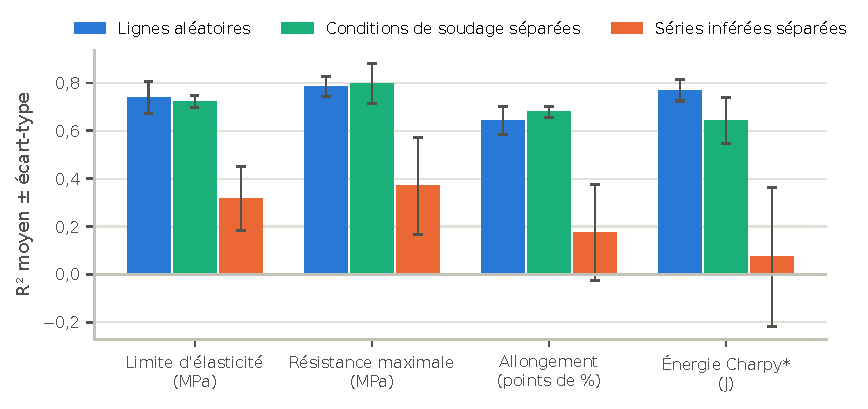
\includegraphics[width=\textwidth]{diag_decoupages_rf}
\caption{Même forêt aléatoire, sans réglage, configuration 16/médiane, sous trois
découpages. Séparer des conditions de soudage répétées change peu le score ;
séparer des séries entières le fait chuter.}
\label{fig:decoupages}
\end{figure}

\begin{table}[htbp]
\centering
\small
\caption{$R^2$ moyen de la forêt fixe selon le découpage, et structure des séries.}
\label{tab:decoupages}
\begin{tabular}{@{}l rrr rr@{}}
\toprule
 & \multicolumn{3}{c}{$R^2$ moyen selon le découpage} & \multicolumn{2}{c}{Structure des séries} \\
\cmidrule(lr){2-4}\cmidrule(lr){5-6}
Cible & Lignes & Conditions & Séries & Séries multi-conditions & Variance entre séries \\
\midrule
\YS     & 0,739 & 0,722 & 0,318 & 37 / 40 & 48,0\,\% \\
\UTS    & 0,786 & 0,797 & 0,370 & 36 / 39 & 54,9\,\% \\
Allong. & 0,644 & 0,680 & 0,175 & 33 / 34 & 54,4\,\% \\
Charpy  & 0,769 & 0,643 & 0,074 & 23 / 24 & 29,1\,\% \\
\bottomrule
\end{tabular}
\end{table}

Pour la traction, séparer les conditions répétées ne fait presque pas baisser le
score : le problème n'est pas une simple répétition de mesures identiques. En
revanche, séparer des séries divise le $R^2$ par deux à quatre. Presque toutes
les séries contiennent plusieurs conditions de soudage (37 sur 40 pour \YS) : ce
ne sont pas des doublons, mais des études cohérentes dont le \og niveau \fg{} est
propre. Un test de permutation (999 permutations) confirme que la part de
variance des cibles portée par les séries (29 à 55\,\%) est très supérieure à ce
qu'on obtiendrait par hasard (4 à 8\,\% au 95\textsuperscript{e} centile ; $p = 0{,}001$).
Ce test reste exploratoire : les répétitions limitent l'échangeabilité des lignes.
Pour Charpy, 65\,\% des points de validation aléatoire partagent la condition de
soudage d'un point du train (à une autre température), ce qui explique son
$R^2$ aléatoire élevé.

\subsection{Quantité de données : courbes d'apprentissage}

La \cref{fig:apprentissage} fait varier la fraction des groupes du train (50, 75 et
100\,\%) sans toucher à la validation, avec deux graines.

\begin{figure}[htbp]
\centering
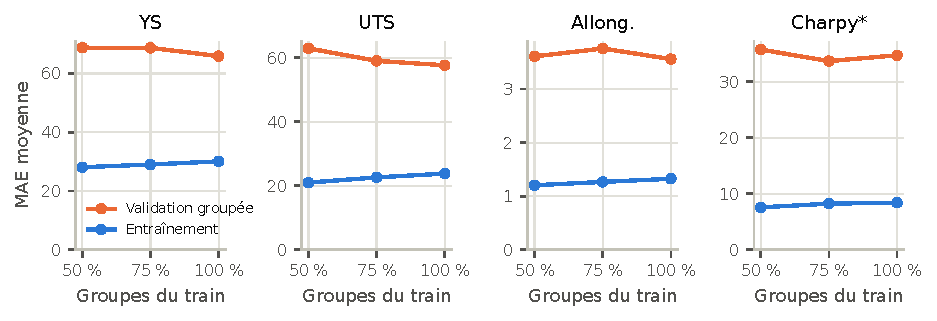
\includegraphics[width=\textwidth]{diag_courbes_apprentissage}
\caption{MAE d'entraînement et de validation groupée de la forêt (benchmark
13/itérative) en fonction de la fraction de groupes d'entraînement utilisée.}
\label{fig:apprentissage}
\end{figure}

\YS{} et \UTS{} profitent de groupes supplémentaires (MAE \UTS{} de 62,9 à
57,7\,MPa), tandis que l'allongement et Charpy ne s'améliorent pas de façon
monotone. Le large écart entre train et validation persiste : davantage de
\emph{séries diverses} semble plus utile que davantage de lignes d'une même série.

\subsection{Explicabilité : quelles informations le modèle utilise-t-il ?}

L'importance par permutation~\cite{breiman_2001,fisher_2019} mesure la hausse de
MAE lorsque l'on mélange aléatoirement une entrée (ou un bloc d'entrées corrélées)
dans la validation, sans réentraîner le modèle. Les blocs sont : composition,
paramètres de soudage, PWHT, procédé et, pour Charpy, température d'essai.

\begin{figure}[htbp]
\centering
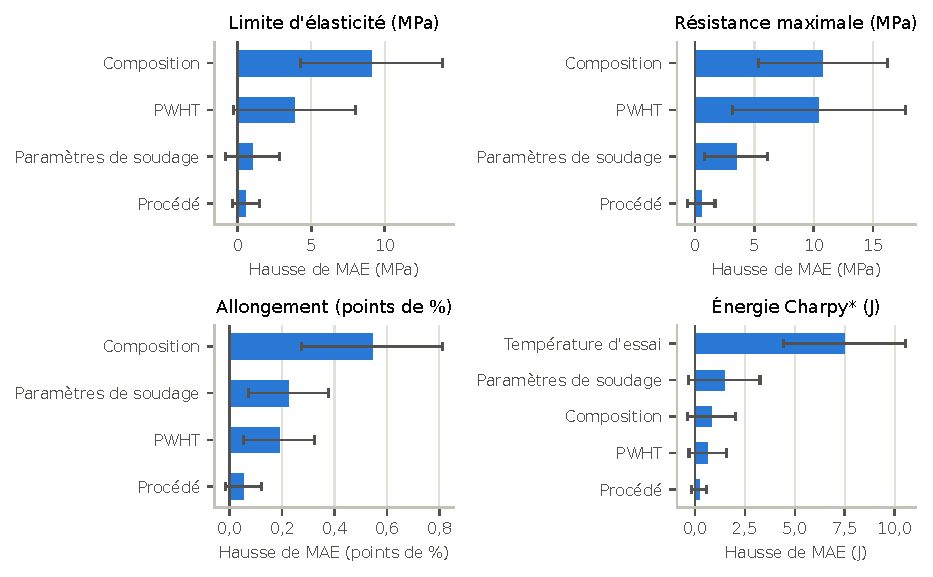
\includegraphics[width=\textwidth]{diag_importance_blocs}
\caption{Importance par permutation de blocs d'entrées (forêt du benchmark
13/itérative, validation groupée, dix permutations par pli). Barres : hausse
moyenne de MAE ; traits : écart-type entre répétitions et plis.}
\label{fig:importance}
\end{figure}

La \cref{fig:importance} indique que la \textbf{composition} et le \textbf{PWHT}
portent l'essentiel de l'information utilisée pour la résistance (hausse de MAE
de 9,1 et 3,9\,MPa pour \YS ; 10,7 et 10,4\,MPa pour \UTS), que la composition
domine pour l'allongement, et que la \textbf{température d'essai} domine pour
Charpy (+7,5\,J). Des contributions locales exactes, calculées le long des chemins
des arbres, reconstruisent chaque prédiction et ont servi à analyser les plus
grosses erreurs ; elles dépendent de l'ordre des coupures et ne sont pas des
valeurs SHAP.

\begin{precaution}
Ces importances décrivent \emph{le comportement du modèle}, pas des effets
physiques causaux. Des entrées corrélées peuvent se substituer l'une à l'autre,
et l'importance d'une variable dans un modèle faible n'établit pas une hiérarchie
métallurgique.
\end{precaution}

\subsection{Audit des protocoles Charpy}
\label{subsec:charpy_audit}

Pour Charpy, les séries ont été confrontées à leurs publications originales,
par correspondance de compositions et de conditions (\cref{tab:charpy_audit}).

\begin{table}[htbp]
\centering
\small
\caption{Correspondance des séries Charpy avec leurs publications originales.}
\label{tab:charpy_audit}
\begin{tabularx}{\textwidth}{@{}l r L@{}}
\toprule
Série & Lignes & Constat \\
\midrule
\texttt{SvenGret-1990}~\cite{svensson_gretoft_1990} & 80 & 16 compositions et conditions concordantes ; énergies mesurées à cinq températures présélectionnées, cinq éprouvettes par température : \textbf{courbes $E(T)$ confirmées} \\
\texttt{Evans-StressRelief-1991}~\cite{evans_1986_sr} & 94 & 16 compositions et six conditions concordantes avec une publication de 1986 (malgré l'année 1991 de l'identifiant) : \textbf{famille de courbes de transition confirmée} \\
\texttt{Evans-Cr/CMn-1989}~\cite{evans_1989_cr} & 31 & 20 compositions concordantes ; la publication présente des températures à 100\,J et les 31 couples valent 100\,J : \textbf{extraction de températures de transition probable} \\
21 autres séries & 656 & Non résolues par leur publication originale \\
\bottomrule
\end{tabularx}
\end{table}

Dans la cohorte, 457 des 861 énergies (53,1\,\%) valent exactement 28 ou 100\,J.
Un point à 100\,J appartient bien à la courbe $E(T)$, mais sa température a été
choisie en fonction de l'énergie : il renseigne la position de la transition,
pas toute la courbe. Mélanger ces règles d'échantillonnage peut modifier la
distribution évaluée. Deux familles confirmées (174 points) ne suffisent pas à
construire une nouvelle validation imbriquée par sources : \textbf{Charpy reste
exploratoire}. L'audit a par ailleurs confirmé que la publication Svensson--Gretoft
exprime Ti/Al/Sn/As/Sb en \% massique, ce qui conforte la quarantaine des unités.

\subsection{Bilan des diagnostics}

\begin{aretenir}
\textbf{Établi :} grand écart train/validation ; environ la moitié de l'erreur
due à des décalages de niveau entre séries ; prédictions comprimées ; apport
réel de Ni/Cr/Mo pour \YS{} et \UTS ; instabilité de l'imputation itérative à
16 entrées ; difficulté accrue hors du domaine du train pour Charpy ; règles
d'échantillonnage Charpy hétérogènes.

\textbf{Plausible mais non isolé :} compositions ou états métallurgiques omis
(Nb, V, Cu, Ti, B\ldots), différences de protocoles entre séries, précision de
transcription des labels.

\textbf{Non démontré :} que l'imputation explique les faibles scores ; qu'un
bruit expérimental plafonne le $R^2$ sous 0,5 ; qu'une ACP ou un modèle
multi-sorties résoudrait le problème ; que retirer les séries difficiles
améliorerait la généralisation.
\end{aretenir}
